\section{Application}

A typical application of Catalan Numbers is counting the number of ways starting from $(0, 0)$ to $(n, n)$ in a $n \times n$ grid without crossing the line $y = x-1$  (figure \ref*{fig:symmetry}).


The general formula and the recurrence formula can be interpreted through this application. The general formula is used to directly calculate the number of ways to reach $(n, n)$ from $(0, 0)$ in a $n \times n$ grid without crossing the line $y = x-1$. The recurrence formula is used to calculate the number of ways to reach point $(n, n)$ from $(0, 0)$ in a $n \times n$ grid without crossing the line $y = x-1$ by using previous number derived from point $(n-1, \ n-1)$.

For general formula, it is clear that the number of ways to reach $(n, n)$ from $(0, 0)$ in a $n \times n$ grid without crossing the line $y = x-1$ is equal to the total number of ways to reach $(n, n)$ from $(0, 0)$ minus the number of ways to reach $(n, n)$ from $(0, 0)$ in a $n \times n$ grid crossing the line $y = x-1$. The Figure~\ref{fig:symmetry} shows to do a symmetry transformation with respect to the line $y = x-1$. Then

\begin{equation}
    C_n = \binom{2n}{n} - \binom{2n}{n-1} = \frac{1}{n+1}\binom{2n}{n}.
\end{equation}

\begin{multicols}{2}
    \begin{figure}[H]
        \centering
        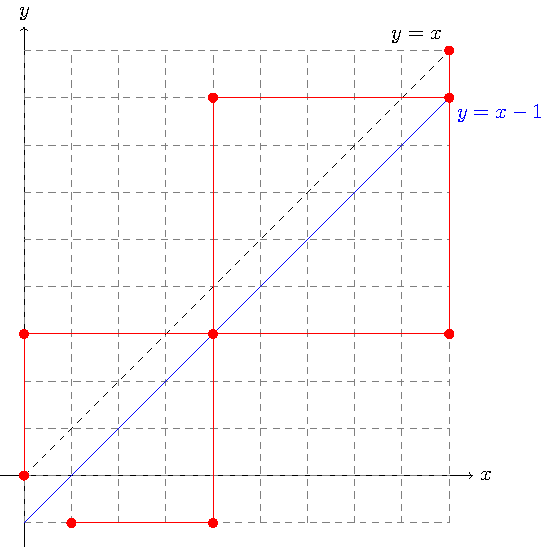
\includegraphics[width=0.9\columnwidth]{figures/symmetry.pdf}
        \caption{general Formula}\label{fig:symmetry}
    \end{figure}
    \begin{figure}[H]
        \centering
        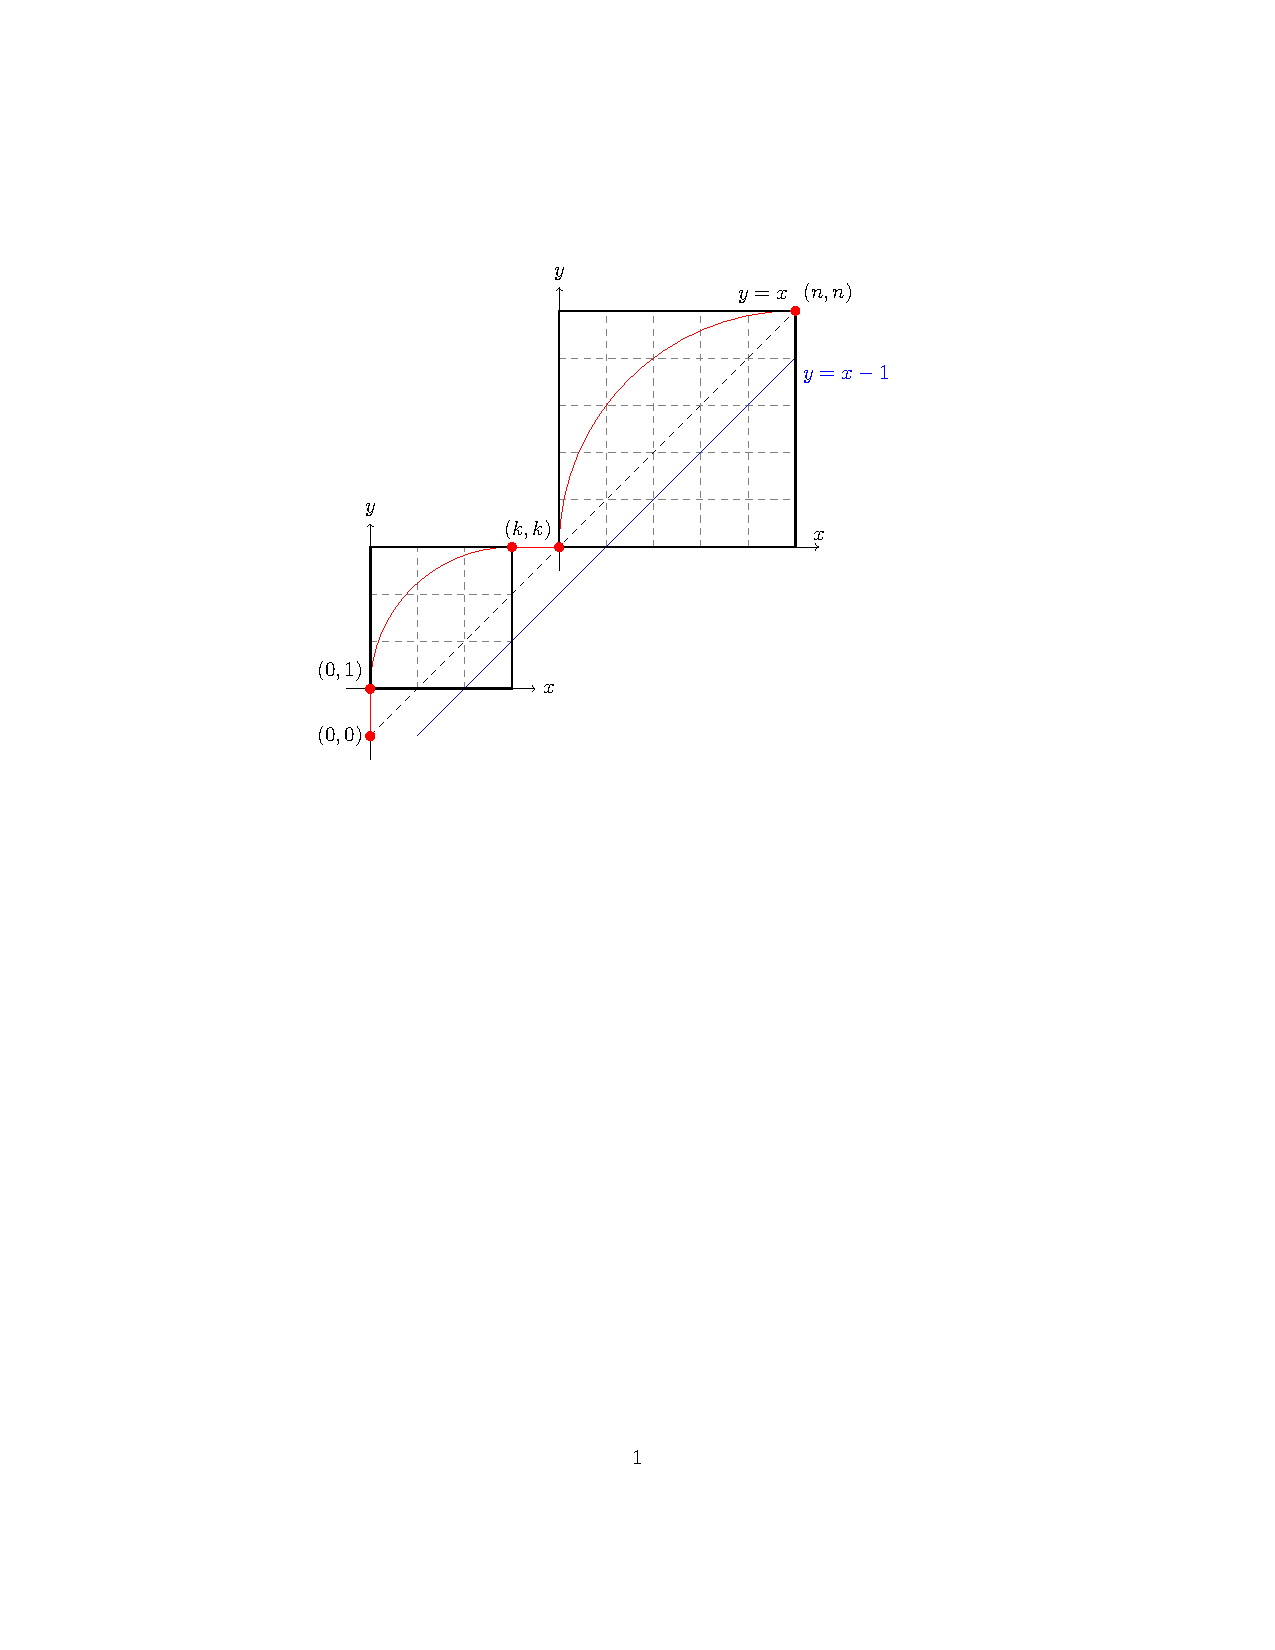
\includegraphics[width=\columnwidth]{figures/recurrence.pdf}
        \caption{recurrence Formula}\label{fig:recurrence}
    \end{figure}
\end{multicols}

For recurrence relation, suppose a point in the moving process touches the line $y=x$ at point $(k,k)$, then the path can be divided into two parts: the first part is from $(0,0)$ to $(k,k)$ (i.e. $(0,1)\to(k-1,k)$), and the second part is from $(k,k)$ to $(n,n)$. By principle of multiplication, the first part will be in $C_k$ ways and the second part will be in $C_{n-1-k}$ ways. Therefore,
\begin{equation}
    C_n = \sum_{k=0}^{n-1} C_kC_{n-1-k}. 
\end{equation}